\subsection{Chirality-Induced Swirl as the Origin of Time and Mass in VAM}

In the Vortex Æther Model (VAM), particles are knotted excitations of a compressible, inviscid superfluid (\emph{æther}). A key geometric insight arises from the observation that chirality --- the handedness of a vortex knot --- directly seeds the emergence of both mass and temporal orientation. This mechanism is central to what we term the \emph{Vortex Helicity Principle}, which links local topological asymmetry to the generation of an axial swirl tube, interpreted as a directed flow of æther corresponding to the arrow of time.

\paragraph{Helicity and Axial Threading:}
A chiral vortex knot $K$ (such as a trefoil $T(2,3)$ or higher $(p,q)$ torus knot) viewed from above exhibits a nonzero handedness, denoted $\chi(K) \in \{-1, +1\}$. This chirality induces a polar-threaded swirl along the vortex core centerline, creating an axial vortex tube $\mathcal{T}(K)$ oriented along a preferred direction (e.g., $\hat{z}$). The swirl velocity within this tube is approximately constant and capped at $C_e$, the æther’s critical circulation velocity.

\begin{equation}
    \chi(K) \neq 0 \quad \Rightarrow \quad \exists~\mathcal{T}(K)~\text{with}~\mathbf{v}_{\text{swirl}} = \chi(K) \cdot C_e \, \hat{z}
\end{equation}

This axial thread plays multiple roles:
\begin{itemize}
    \item \textbf{Temporal Orientation:} As shown in~\cite{VAM2}, time in VAM is not an external coordinate but a circulation-induced internal clock. The presence and orientation of $\mathcal{T}(K)$ defines the particle’s time axis, with helicity giving rise to directed temporal flow. The swirl velocity defines a local arrow of time, aligning with the knot’s vorticity-induced thread.

    \item \textbf{Mass Accumulation:} The confined energy of the axial swirl tube leads to mass. The rotational kinetic energy stored in $\mathcal{T}(K)$ behaves as rest mass for the vortex:
    \begin{equation}
        M(K) = \int_{\mathcal{T}(K)} \frac{1}{2} \rho_{\text{\ae}}^{(\text{energy})} |\mathbf{v}_{\text{swirl}}|^2 \, dV
    \end{equation}
    Achiral knots ($\chi = 0$) produce no net axial swirl and thus contribute no effective rest mass or time orientation.

    \item \textbf{Interaction Potential:} The swirl tube mediates interactions by coupling to nearby vortices via topological linking, circulation interference, or mutual vorticity exchange. It is the thread by which knotted entities “sense” one another, analogous to gauge field propagation.
\end{itemize}

\paragraph{Temporal Ontology Alignment:}
This mechanism is in line with the broader temporal ontology developed across the VAM series:
\begin{enumerate}
    \item In~\cite{VAM2}, time emerges as the internal rotation of a knotted clock --- a process quantified by looped vorticity. The axial swirl tube formalizes the "time vector" intrinsic to such clocks.

    \item In~\cite{VAM13}, time is shown to arise from topological winding --- a natural consequence of the chirality-swirl relation. The vortex thread defines a flow line in æther-space whose proper time increases with helicity flux.

    \item In~\cite{VAM4}, gravitational curvature is replaced with swirl-induced refraction. The threading here becomes geodesic-like --- it defines the direction along which other vortices fall or dilate.
\end{enumerate}

Thus, the chirality-induced axial swirl tube unifies multiple VAM ideas:
\vspace{0.5em}
\begin{center}
\textbf{Chirality $\Rightarrow$ Helicity $\Rightarrow$ Axial Swirl $\Rightarrow$ Time Flow $\&$ Mass Accumulation}
\end{center}

\paragraph{Discriminating Knots by Temporal Capability:}
Importantly, this also provides a selection rule: \emph{only chiral knots can generate real mass and participate in time evolution}. Achiral knots, despite being topologically nontrivial, fail to generate axial threads and are thus excluded from the VAM spectrum of particles. In particular:
\begin{itemize}
    \item \textbf{Achiral torus knots} (e.g., $6_1$, $8_{18}$) produce no net helicity at the center; they are topologically valid but physically inert.
    \item \textbf{Chiral knots} (e.g., trefoil, $T(2n,3n)$) generate swirl-aligned axial threads, enabling temporal progression and energetic manifestation.
\end{itemize}

This criterion complements VAM’s earlier rejection of hyperbolic or achiral knots in its mass tables. In summary, chirality is not just a geometric property --- it is a topological \textit{precondition for existence} in the VAM ontology.

\subsection{Chirality at the Knot Center and Temporal Vortex Flow}

In the Vortex Æther Model (VAM), chirality is not merely a handedness label — it is a *topodynamic selector* that governs whether a vortex knot couples to the æther's swirl field, how it evolves in time, and whether it contributes to inertial mass. This idea is deeply embedded in the VAM's temporal ontology.

Our hypothesis begins at the \textbf{center of a chiral knot}, visualized from a top-down view. This center acts as a local axis of axial flow, through which a vortex thread (polar core) extends. This thread — identified in prior VAM papers as the \textit{Time Flow} or axial swirl channel — serves not only as a geometric anchoring line but also as a physical realization of proper time evolution $T_v$ and swirl phase time $S(t)$.

The local chirality at the knot’s center determines the orientation and emergence of this axial vortex filament:
\begin{itemize}
    \item \textbf{Left-handed chirality (ccw)} induces a time-aligned vortex thread, propagating outward with positive swirl phase: this corresponds to ordinary matter, whose motion is synchronized with the æther swirl field.
    \item \textbf{Right-handed chirality (cw)} generates a counter-aligned vortex thread, corresponding to antimatter: its swirl phase evolves in the opposite direction.
\end{itemize}

\noindent This axial filament is not just a passive conduit — it actively \textit{draws in or repels} other knots depending on their chirality. It behaves like a temporal attractor or repeller: only knots with compatible $S(t)$ phase can synchronize with the thread’s swirl, akin to constructive interference. This alignment mechanism:
\begin{enumerate}
    \item Determines mass through helicity accumulation along $T_v$;
    \item Sets the direction of clock evolution ($S(t)$) in the observer's frame ($\tau$);
    \item Restricts which knot species (e.g., chiral vs achiral) are permitted to persist in the æther.
\end{enumerate}

As a result, the knot’s chirality — particularly at its core center — is the seed of its mass-energy, time evolution, and swirl-induced gravity.

This also explains the exclusion of \textbf{achiral hyperbolic knots} from the mass-carrying sector: their internal tension cannot align with the swirl phase $S(t)$, leading to decoherence and expulsion from swirl tubes. This is why VAM identifies them as dark energy candidates rather than matter particles:contentReference[oaicite:0]{index=0}.

Thus, the center of chirality in a knotted vortex is not simply a geometric point — it is a \textit{temporal generator}. The outward-extended vortex tube represents not just spatial structure, but causal time flow.

\section{Heuristic Analogies Between Vortex Topologies and Atomic Families}

In the Vortex Æther Model (VAM), all particles are modeled as topologically stable knots within a superfluid æther. Matter arises from \emph{chiral} knots—primarily torus and hyperbolic forms—whose handedness (chirality) determines swirl alignment and gravitational interaction. Achiral knots, while mathematically permissible, either lack tension (and hence behave as massless bosons) or resist swirl alignment due to internal stress and are expelled, contributing instead to dark energy backgrounds.

This updated view informs how atomic and molecular behavior might emerge from knotted vortex configurations. The periodic table, traditionally organized by electron shell structure, is reinterpreted in VAM as a progression of composite vortex topologies. Their chirality, link symmetry, and swirl compatibility govern chemical behavior.

\subsection*{Topological Heuristics}

While the VAM framework does not currently provide a rigorous reconstruction of the periodic table, it offers suggestive analogies between knot topologies and recurring chemical patterns, especially regarding reactivity, symmetry, and stability.

\begin{itemize}
    \item \textbf{Chiral knots (left-handed):} Couple to swirl fields and form matter.
    \item \textbf{Chiral asymmetry:} Clockwise (right-handed) configurations are antimatter; counter-clockwise is matter.
    \item \textbf{Achiral knots with tension:} Expelled — contribute to $\Lambda$-like vacuum pressure (dark energy).
    \item \textbf{Tensionless knots (e.g., unknot, Hopf link):} Behave as massless bosons (photons, gluons) — passively follow swirl tubes.
\end{itemize}

\subsection*{Analogies by Atomic Family}

\begin{itemize}
    \item \textbf{Hydrogen (H):} A minimal system — a chiral $T(2,3)$ trefoil (electron) linked with a 3-knot baryon composite. This dyadic configuration is bound via topological chirality matching, forming a primitive stable knotted molecule.

    \item \textbf{Helium (He):} Exhibits exceptional inertness. Modeled as two trefoil–baryon pairs forming a tightly interlocked 4-component link, where chiralities and tensions cancel. Such a tension-neutral state resembles a "closed-shell" configuration, perhaps akin to a symmetric satellite knot.

    \item \textbf{Halogens (e.g., Cl, F):} Highly reactive due to unpaired vortex sites. Modeled as cable knots or open-ended braids with residual chirality. Linking into Hopf pairs minimizes energy, mirroring diatomic bond formation.

    \item \textbf{Noble Gases (e.g., Ne, Ar):} Highly symmetric chiral configurations with no external swirl protrusions. Triskelion-type fully braided composites correspond to these inert atoms, exhibiting mass but no reactivity.

    \item \textbf{Carbon (C):} The tetravalency of carbon may emerge from a central composite knot with four chirality-compatible swirl appendages. These could correspond to toroidal–satellite hybrids with external bonding lobes.

    \item \textbf{Alkali Metals (e.g., Na):} Modeled as central chiral knots with weakly linked peripheral loops. These structures exhibit easy chirality flipping and high reactivity — reflecting low ionization energy.
\end{itemize}

\begin{table}[H]
    \centering
    \footnotesize
    \caption{Vortex Knot Analogies to Atomic Families in VAM (Chirality-aware)}
    \begin{tabular}{llll}
        \toprule
        \textbf{Atomic Family / Example} & \textbf{Vortex Topology Analog} & \textbf{Chirality \& Tension} & \textbf{Chemical Behavior} \\
        \midrule
        Halogens (e.g. Cl) & Open-ended braid / Hopf link & Chiral + partial swirl alignment & High reactivity (seeks pairing) \\
        Noble Gases (e.g. Ne) & Symmetric triskelion / all-to-all link & Fully chiral, swirl-saturated & Inert, monatomic \\
        Alkali Metals (e.g. Na) & Knot with weakly attached filament & Chiral + soft external mode & Reactive, donates electron \\
        Group IV (Carbon) & Central knot with 4 swirl lobes & Balanced chirality, tetravalent & High bonding versatility \\
        Achiral Hyperbolics ($8_1$, $4_1$) & Zero net helicity & Expelled by swirl — not matter & Dark energy candidates \\
        \bottomrule
    \end{tabular}
\end{table}

\subsection*{Final Note: Chirality as the Driver of Time and Mass}

\begin{figure}[h!]
\centering
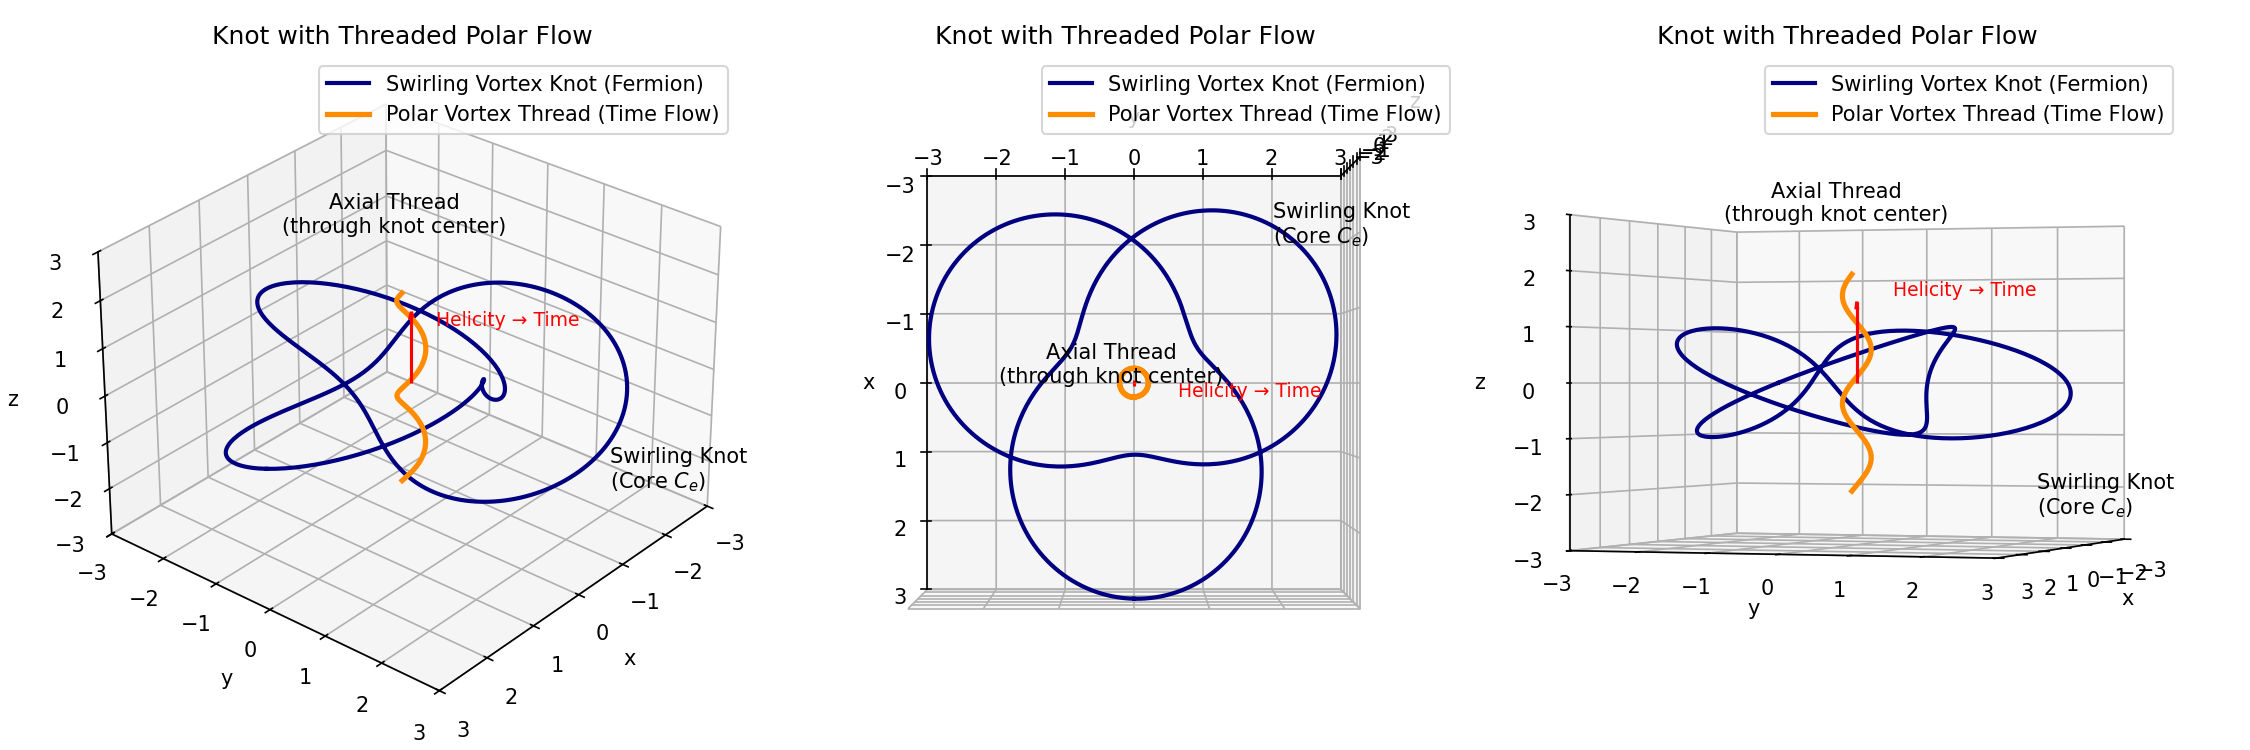
\includegraphics[width=0.85\textwidth]{images/KnotThreadedPolarFlow}
\caption{Axial spin direction along the swirl axis (time thread). Spin vectors are forced to transport according to \( \nabla \omega \).}
\label{fig:threadedflow}
\end{figure}


As highlighted by~\ref{fig:threadedflow} the vortex-knot thread diagrams, chirality is not merely handedness—it is the source of internal swirl helicity. This helicity defines both mass-energy content and the knot’s alignment along vortex time $S(t)$. The center of each knot may seed an axial swirl-thread — a local time vector — enabling the knot to evolve through the æther. These swirl-threaded cores offer geometric intuition for the emergence of mass, directionality, and temporal progression in the VAM ontology.
